\section{Durchführung}
Zunächst wurde bei der nach \autoref{fig:Abb1} gebaute Schaltung die Frequenz des Generators auf die Resonanzfrequenz des Systems gestellt, sodass der Energieabtausch zwischen beiden gekoppelten Schwingkreisen vollständig erfolgen konnte. Der Theoriewert dieser Frequenz wurde zuerst durch das Einsetzen der Werte der Kapazität des Kondensators \(C\) (0,037 nF), sowie die des Kondensators \(C_{sp}\) (0,8015 nF), als auch die der Induktivität der Spule \(L\) (32,351 mH) in die Thomson'sche Schwingungsgleichung. Auf die Weise wurde die Unsicherheit des zu durchführenden Experiments ermittelt, bzw. eher veranschaulicht.
\\
Als nächstes wurde die Schaltung nach \autoref{fig:Abb2} nachgebaut. Die Erregung des linken Schaltkreises erfolgte mithilfe eines Rechteckimpulses, während der rechte nur indirekt durch den linken Schaltkreis selber angeregt werden durfte. Auf dem Oszilloskop werden daraufhin die Anzahl aller Schwingungsextrema innerhalb einer Schwingungsperiode abgezählt. Das Prozedere wird nochmal mit allen Werten des Koppelkondensators \(C_k\). Der Zweck dessen war es das Verhältnis zwischen Schwingungs- und Schwebungsfrequenz herauszufinden. 
\\
Hinterher sollen die Frequenzen \(v^-\) und \(v^+\) in Abhängigkeit von \(C_k\) experimentell ermittelt werden, indem die bisherige Schaltung weiterhin genutzt und nun statt Rechteck- der Sinusgenerator benutzt wird. Nach jeder Umstellung des Doppelkondensators wurden die Lissajous-Figren benutzt, um die Phasen auf 0 zu setzen. 
\\
Zum Schluss wurde der Schaltkreis gemäß \autoref{fig:Abb3} aufgebaut. Um den Verlauf der Ströme \(I_2\) und \(I_k\) zu messen, wurde mit dem AC-Breitband-Millivoltmeter und dem Wobbelgenerator ein Gleichspannungssignal durch das System geschickt. Mitsamt der vom Wobbelgenerator erzeugten Wechselspannung konnte nun der Strom in Abhängigkeit von einer sinkenden Frequenz aufgetragen werden, dessen Startwert 24,99 Hz und Endwert 50,85 Hz waren, welche in einem Zeitintervall von 0,16 Sekunden durchlaufen wurden. Das Resultat war ein kleiner und 2 große Peaks auf dem Oszillographen \autoref{fig:Abb4}. Zunächst wurde der Abstand zwischen dem ersten großen und den kleinen Peak gemessen. Daraufhin die Amplitude des ersten großen Peaks. Dasselbe folgte für den ersten und zweiten großen Peak. Für jedes einzelne \(C_k\) wurden diese Messungen durchgeführt.
\begin{figure}
    \centering
    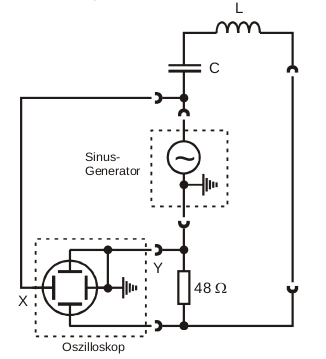
\includegraphics[scale=0.7]{content/Bilder/Test.png}
    \caption{Schaltung zur experimentellen Ermittlung der Resonanzfrequenz.}
    \label{fig:Abb1}
    \end{figure}
    \begin{figure}
        \centering
        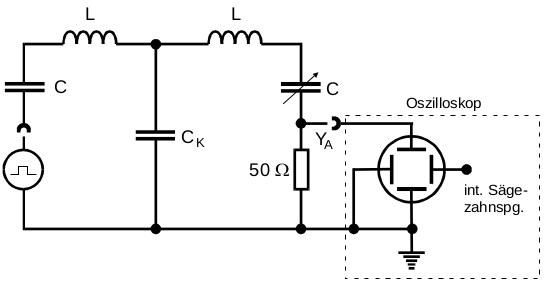
\includegraphics[scale=0.7]{content/Bilder/a_b.png}
        \caption{Schaltung zur experimentellen Ermittlung des Verhältnisses zwischen Schwingungs- und Schwebungsfrequenz.}
        \label{fig:Abb2}
        \end{figure}
\begin{figure}
    \centering
    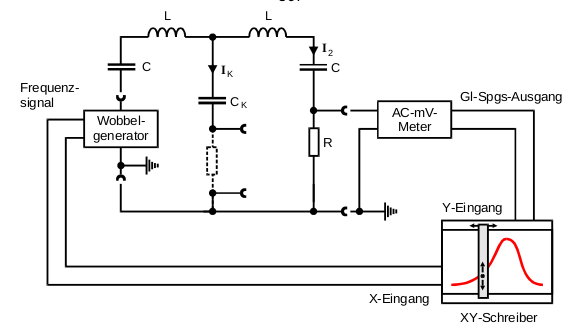
\includegraphics[scale=0.7]{content/Bilder/c.png}
    \caption{Schaltung zur experimentellen Ermittlung des Stroms.}
    \label{fig:Abb3}
    \end{figure}

    \begin{figure}
        \centering
        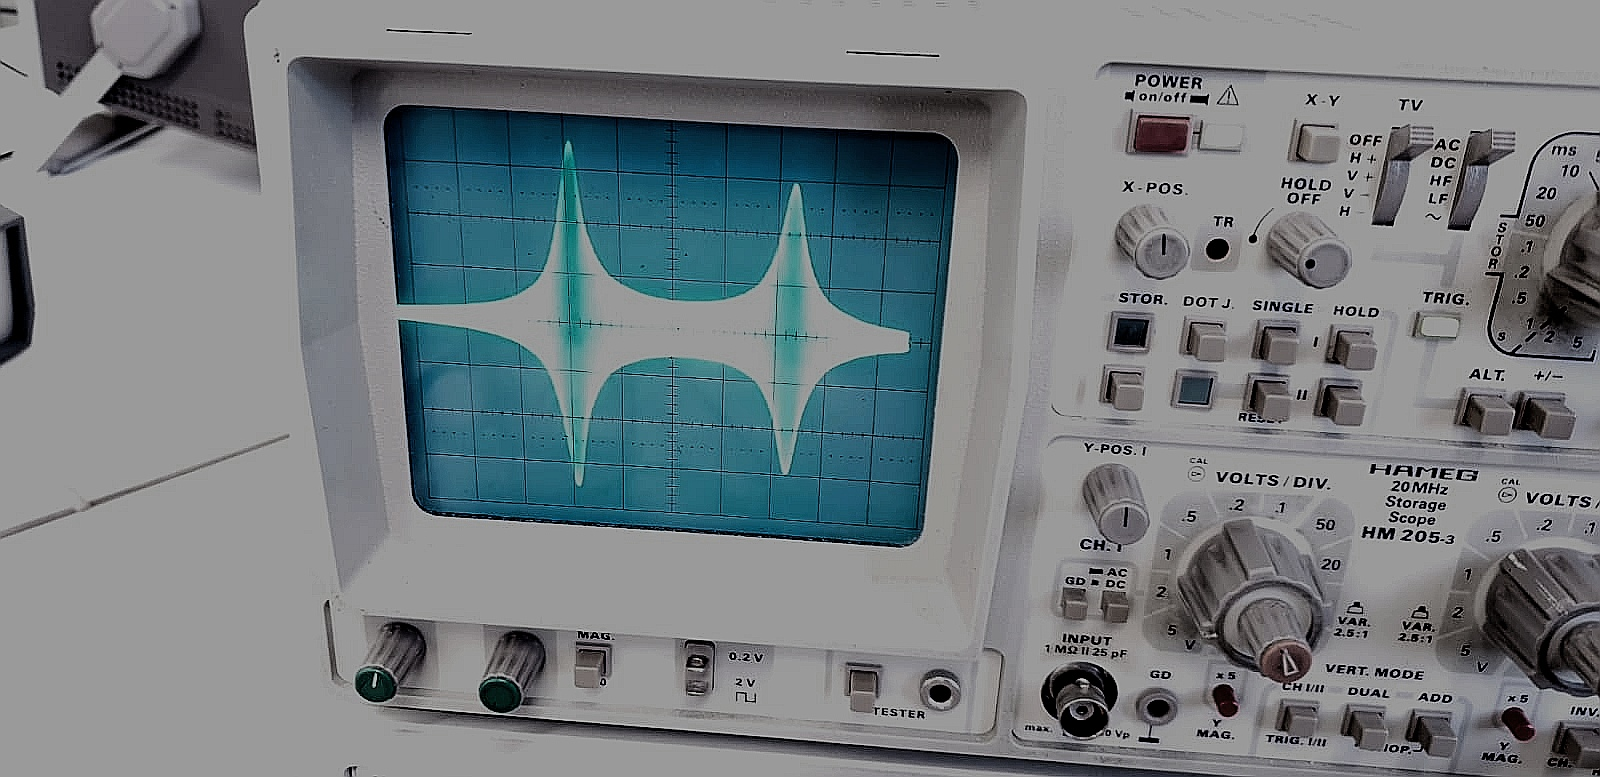
\includegraphics[scale=0.09]{content/Bilder/Titelbild.jpg}
        \caption{Der Strom des Schaltkreises bei einer sich andauernd wiederholenden sinkenden Frequenz.}
        \label{fig:Abb4}
        \end{figure}
\label{sec:Durchfuehrung}
